\documentclass[a4paper,12pt,twoside]{report}
%\usepackage[Danish]{babel}
%\usepackage[utf8]{inputenc}
%\usepackage{fancyhdr}
%Gør det muligt at bruge \pagestyle{fancyplain}
%\usepackage[backend = bibtex]{biblatex}
%\addbibresource{myBilag.bib} %Bilags filen

\usepackage{epstopdf}

%%%%%
%%%%%%%%%%%%%%%%%%%%%%%%%%%%%%%%%%%%%%%%%%%%%%%%
% Language, Encoding and Fonts
% http://en.wikibooks.org/wiki/LaTeX/Internationalization
%%%%%%%%%%%%%%%%%%%%%%%%%%%%%%%%%%%%%%%%%%%%%%%%
% Select encoding of your inputs. Depends on
% your operating system and its default input
% encoding. Typically, you should use
%   Linux  : utf8 (most modern Linux distributions)
%            latin1 
%   Windows: ansinew
%            latin1 (works in most cases)
%   Mac    : applemac
% Notice that you can manually change the input
% encoding of your files by selecting "save as"
% an select the desired input encoding. 
\usepackage[utf8]{inputenc}
% Make latex understand and use the typographic
% rules of the language used in the document.
\usepackage[Danish]{babel}
% Use the palatino font
\usepackage[sc]{mathpazo}
\linespread{1.05}         % Palatino needs more leading (space between lines)
% Choose the font encoding
\usepackage[T1]{fontenc}
%%%%%%%%%%%%%%%%%%%%%%%%%%%%%%%%%%%%%%%%%%%%%%%%
% Graphics and Tables
% http://en.wikibooks.org/wiki/LaTeX/Importing_Graphics
% http://en.wikibooks.org/wiki/LaTeX/Tables
% http://en.wikibooks.org/wiki/LaTeX/Colors
%%%%%%%%%%%%%%%%%%%%%%%%%%%%%%%%%%%%%%%%%%%%%%%%
% load a colour package
\usepackage{xcolor}
%\definecolor{aaublue}{RGB}{33,26,82}% dark blue
% The standard graphics inclusion package
\usepackage{graphicx}
% Set up how figure and table captions are displayed
\usepackage{caption}
\captionsetup{%
  font=footnotesize,% set font size to footnotesize
  labelfont=bf % bold label (e.g., Figure 3.2) font
}
% Make the standard latex tables look so much better
\usepackage{array,booktabs}
% Enable the use of frames around, e.g., theorems
% The framed package is used in the example environment
\usepackage{framed}

%%%%%%%%%%%%%%%%%%%%%%%%%%%%%%%%%%%%%%%%%%%%%%%%
% Mathematics
% http://en.wikibooks.org/wiki/LaTeX/Mathematics
%%%%%%%%%%%%%%%%%%%%%%%%%%%%%%%%%%%%%%%%%%%%%%%%
% Defines new environments such as equation,
% align and split 
\usepackage{amsmath}
% Adds new math symbols
\usepackage{amssymb}
% Use theorems in your document
% The ntheorem package is also used for the example environment
% When using thmmarks, amsmath must be an option as well. Otherwise \eqref doesn't work anymore.
\usepackage[framed,amsmath,thmmarks]{ntheorem}

%%%%%%%%%%%%%%%%%%%%%%%%%%%%%%%%%%%%%%%%%%%%%%%%
% Page Layout
% http://en.wikibooks.org/wiki/LaTeX/Page_Layout
%%%%%%%%%%%%%%%%%%%%%%%%%%%%%%%%%%%%%%%%%%%%%%%%
% Change margins, papersize, etc of the document
\usepackage[
  inner=28mm,% left margin on an odd page
  outer=41mm,% right margin on an odd page
  ]{geometry}
% Modify how \chapter, \section, etc. look
% The titlesec package is very configureable
\usepackage{titlesec}
\titleformat{\chapter}[display]{\normalfont\huge\bfseries}{\chaptertitlename\ \thechapter}{20pt}{\Huge}
\titleformat*{\section}{\normalfont\Large\bfseries}
\titleformat*{\subsection}{\normalfont\large\bfseries}
\titleformat*{\subsubsection}{\normalfont\normalsize\bfseries}
%\titleformat*{\paragraph}{\normalfont\normalsize\bfseries}
%\titleformat*{\subparagraph}{\normalfont\normalsize\bfseries}

% Clear empty pages between chapters
\let\origdoublepage\cleardoublepage
\newcommand{\clearemptydoublepage}{%
  \clearpage
  {\pagestyle{empty}\origdoublepage}%
}
\let\cleardoublepage\clearemptydoublepage

% Change the headers and footers
\usepackage{fancyhdr}
\pagestyle{fancy}
\fancyhf{} %delete everything
\renewcommand{\headrulewidth}{0pt} %remove the horizontal line in the header
\fancyhead[RE]{\small\nouppercase\leftmark} %even page - chapter title
\fancyhead[LO]{\small\nouppercase\rightmark} %uneven page - section title
\fancyhead[LE,RO]{\thepage} %page number on all pages
% Do not stretch the content of a page. Instead,
% insert white space at the bottom of the page
\raggedbottom
% Enable arithmetics with length. Useful when
% typesetting the layout.
\usepackage{calc}

%%%%%%%%%%%%%%%%%%%%%%%%%%%%%%%%%%%%%%%%%%%%%%%%
% Bibliography
% http://en.wikibooks.org/wiki/LaTeX/Bibliography_Management
%%%%%%%%%%%%%%%%%%%%%%%%%%%%%%%%%%%%%%%%%%%%%%%%
\usepackage[backend=bibtex,
  bibencoding=utf8
  ]{biblatex}
\addbibresource{bib/myKildeliste}

%%%%%%%%%%%%%%%%%%%%%%%%%%%%%%%%%%%%%%%%%%%%%%%%
% Misc
%%%%%%%%%%%%%%%%%%%%%%%%%%%%%%%%%%%%%%%%%%%%%%%%
% Add bibliography and index to the table of
% contents
\usepackage[nottoc]{tocbibind}
% Add the command \pageref{LastPage} which refers to the
% page number of the last page
\usepackage{lastpage}
% Add todo notes in the margin of the document
\usepackage[
%  disable, %turn off todonotes
  colorinlistoftodos, %enable a coloured square in the list of todos
  textwidth=\marginparwidth, %set the width of the todonotes
  textsize=scriptsize, %size of the text in the todonotes
  ]{todonotes}

%%%%%%%%%%%%%%%%%%%%%%%%%%%%%%%%%%%%%%%%%%%%%%%%
% Hyperlinks
% http://en.wikibooks.org/wiki/LaTeX/Hyperlinks
%%%%%%%%%%%%%%%%%%%%%%%%%%%%%%%%%%%%%%%%%%%%%%%%
% Enable hyperlinks and insert info into the pdf
% file. Hypperref should be loaded as one of the 
% last packages
\usepackage{hyperref}
\hypersetup{%
	pdfpagelabels=true,%
	plainpages=false,%
	pdfauthor={Author(s)},%
	pdftitle={Title},%
	pdfsubject={Subject},%
	bookmarksnumbered=true,%
	colorlinks=false,%
	citecolor=black,%
	filecolor=black,%
	linkcolor=blue,% you should probably change this to black before printing
	urlcolor=black,%
	pdfstartview=FitH%
}
\begin{document}
\newcounter{totalp}
\pagenumbering{gobble}
\thispagestyle{empty}
\begin{titlepage}
\begin{nopagebreak}
{\samepage
\begin{tabular}{lr}
\parbox{14.5cm}{
  {\LARGE Dania}

  {\small Academy of Higher Education}
  \vspace{-0.3cm}\\
\hrule
\vspace{0.2cm}
  {\bf Academy Profession (AP) Degree in Computer Science}
 }   & \hspace{-2.8cm} {  
\includegraphics[width=23mm]{pictures/dania}}
\end{tabular}
  

\begin{tabular}{cc}
\parbox{8cm}{
\hspace{2cm}
\begin{description}

\item {\bf TITLE: MMO og systemudvikling mht. drift} 

%  \reporttitle

\end{description}

\parbox{8cm}{

\begin{description}
\item {\bf PROJECT PERIOD:}\\
%Dato for projektet
  Grn14dat2a, \\
  February d. 17, 2016 - Marts d. 4, 2014\\
  \hspace{4cm}
\item {\bf PROJECT GROUP:}\\
%Projekt gruppenummer
  15\\
  \hspace{4cm}
\item {\bf STUDENTS:}\\
%Navne på gruppemedlemmer
  Thomas Harald Marinussen\\
  Morten Henning Jensen\\
  Nicolai Bülov Nielsen\\  
  \hspace{2cm}
\item {\bf SUPERVISOR:}\\
%Navn på vejleder
  Palle Rosendahl Ehmsen\\
\end{description}
}
\begin{description}
%\item{ {\bf COPIES:} 3}
\item{ {\bf REPORT PAGES:} \pageref{lastpage} }
%\item{ {\bf REPORT PAGES:} \pageref{lastreportpage} }
\item{ {\bf APPENDIX PAGES:} \pageref{lastappendixpage} }
\item{ {\bf TOTAL PAGES:} \pageref{totalpages} }
\item{ {\bf TOTAL CHARS:} %Antal af anslag i rapporten 
}
\end{description}
\vfill }
\parbox{7cm}{
  \vspace{.15cm}
  \flushright
  \fbox{
    \parbox{6.5cm}{{\bf ABSTRACT:}\vspace{0.5cm}
     {\vfill{\small{ %myAbstract}
     }}\vspace{0.3cm}
     }
     }
     }
\end{tabular}
}
\end{nopagebreak}
\end{titlepage}

\tableofcontents %Indsætter indholdsfortegnelsen

\clearpage
\pagenumbering{arabic} %Sætter sidetallet til 1
\setcounter{page}{1}

\pagestyle{fancyplain}
\lhead{\thepage}
\rhead{\leftmark}

\cfoot{\page\textbackslash \totalp} %Skal vise x antal sider af y
%\setcounter{page}{1}
\chapter{Hvad er et MMO?}

MMO er en selvstændig verden, forstået på den måde, at verdenen udvikler sig uden der behøver, at være indblanding fra spillere. Det er et online spil, som kan holde til at mange spillere, der kan spille på samme tid i den samme verden\cite{Techopedia}. MMO spil kan blive fundet og spillet på de fleste enheder med adgang til internettet, og er derfor ikke begrænset til én platform, men kan findes til både PC, konsoller og endda telefoner. Hvis man spiller et MMO ved man ikke hvor de andre personer man spiller med er fra, da folk fra hele verdenen kan spille online spil. Typiske mål i et online spil er enten at arbejde sammen om at klare en opgave, eller kæmpe mod hinanden for at vinde som et hold, eller enkeltperson. Der er mange genrer inden for MMO spil, det mest succesfulde er et MMORPG (Massive Multiplayer Online Role Playing Game)\cite{Massively} (Baseret på indtjening)\cite{MMOs}. Der findes flere genrer end MMORPG, som er succesfulde inden for MMO genren\cite{MMORPG}, som dog ikke vil blive uddybet yderligere.
\cfoot{\page\textbackslash \totalp} %Skal vise x antal sider af y
\setcounter{page}{1}
\chapter{Hvor Massive er Massive?}

Et af kendetegnene ved et MMO er antallet af spillere, som kan spille et spil på samme tid, i det samme miljø, men hvor er grænsen for, hvornår et spil går fra at være et multiplayer spil, til at være et massive multiplayer spil? Hvis man ser på spil, som har rigtig mange spillere, som for eksempel League of Legends(LoL)\cite{LoL} eller Counter Strike(CS)\cite{CS}, så mener vi ikke, baseret på vores definition af hvad et MMO er, at disse to spilgenre eksempler (henholdsvis MOBA og FPS) kan gå inden for MMO-genren. Grunden hertil er, at selvom der er mulighed for, at kunne spille et spil med alle andre spillere, så skal man lave et seperat miljø (verden), som kun er tilgængeligt for bestemte og/eller et mindre antal af spillere.
Eftersom begge spil (LoL og CS) har et stort community af spillere og under definitionen af massive \cite{Statistics}, er antallet af spillere og dermed godt kan gå ind under MMO, baseret på det grundlag , så vælger vi at frasortere disse og fokusere på MMO-spil som holder sig inden for vores definition.

Vores konklusion på emnet er, hvis man er mange som kan spille sammen, på samme server(verden/miljø), vil dette kunne kaldes for et MMO.
\chapter{Udviklingsmetoder}
For at få et bedre overblik over, hvilken metode der vil være bedst til at styre driften for et MMO, er det relevant at kigge på forskellige udviklingsmetoder. I følgende afsnit, vil der blive kigget nærmere på metoderne; Vandfaldsmodellen, SCRUM og Unified Process(UP). Hvert afsnit vil indeholde en kort beskrivelse, samt nogle af de fordele og ulemper der er ved at bruge metoden.\\
%\floatBarrier
\section{Vandfaldsmodellen}
Vandfaldsmodellen er en iterativ udviklingsmetode, der er simpel og let anvendelig.\cite{Waterfall} 
Navnet udspringer af den måde, som metoden gennemgår sine seks faser på, som kan ses i figur \ref{dia:Vandfald}.\\

\begin{figure}[!h]
\centering
\begin{center}
%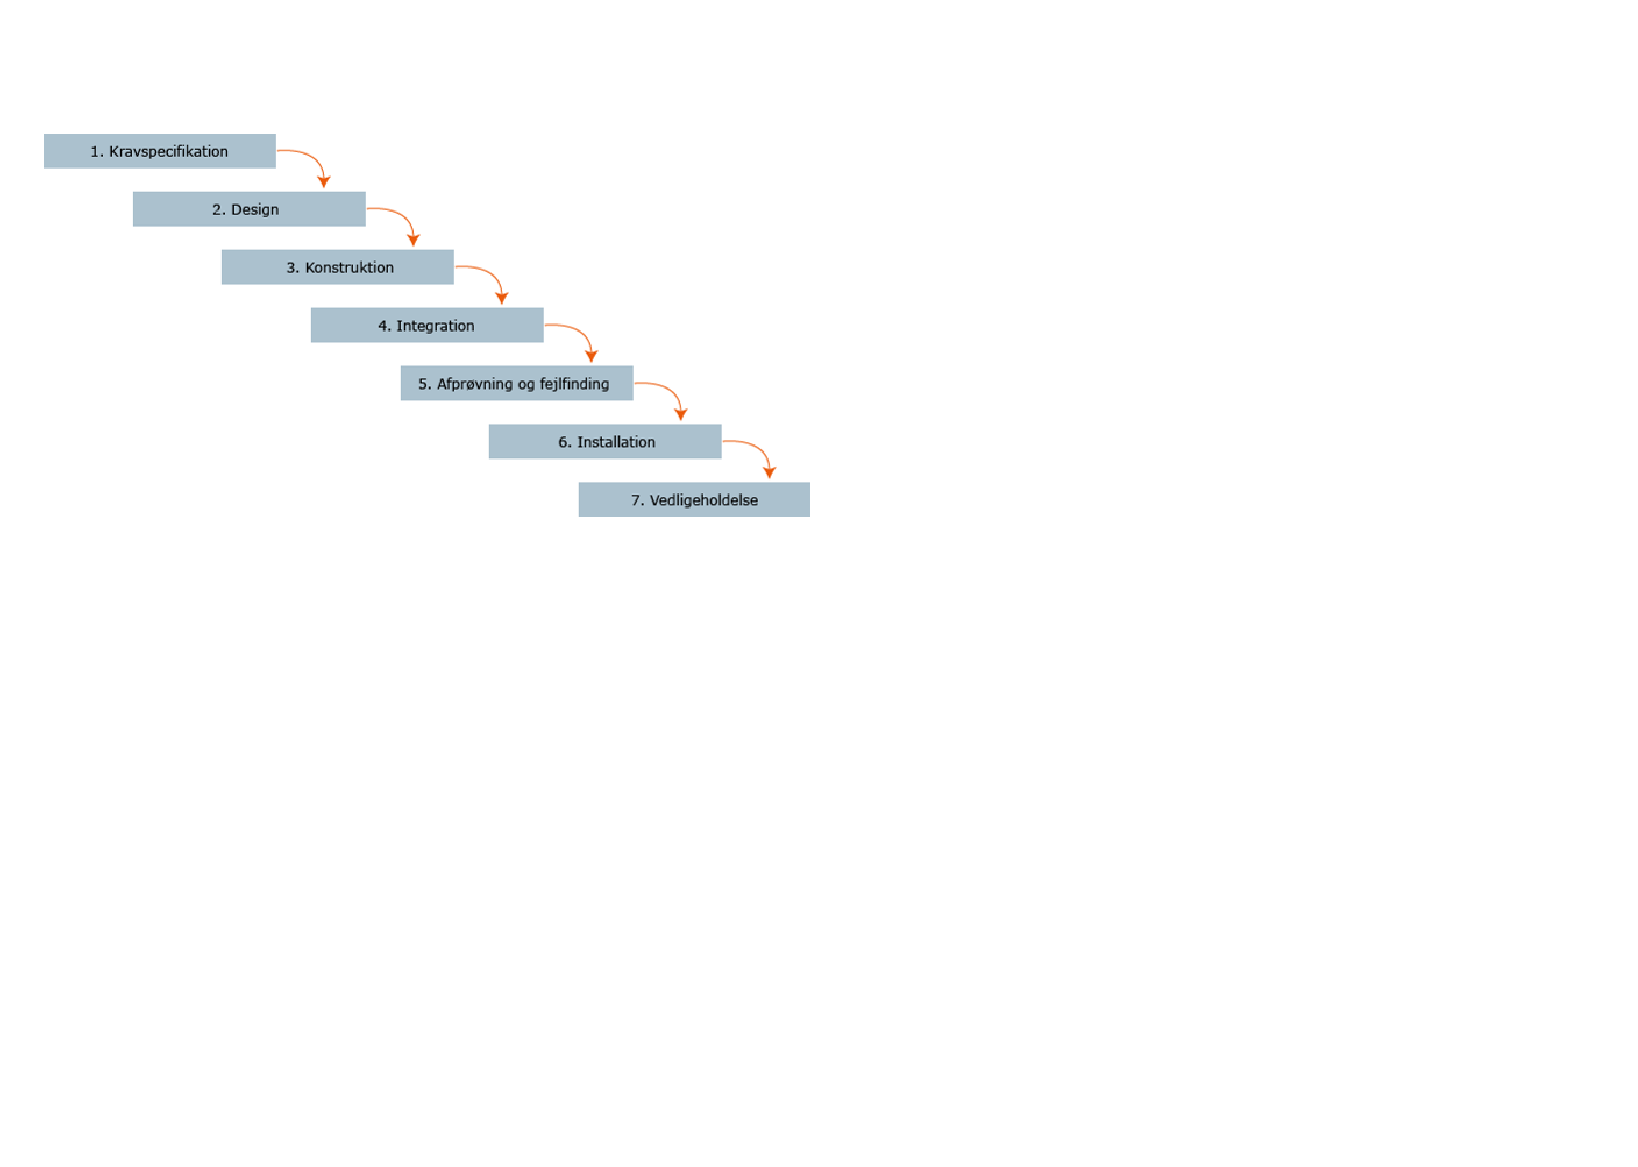
\includegraphics[scale=0.5]{./vandfaldmodel.eps}
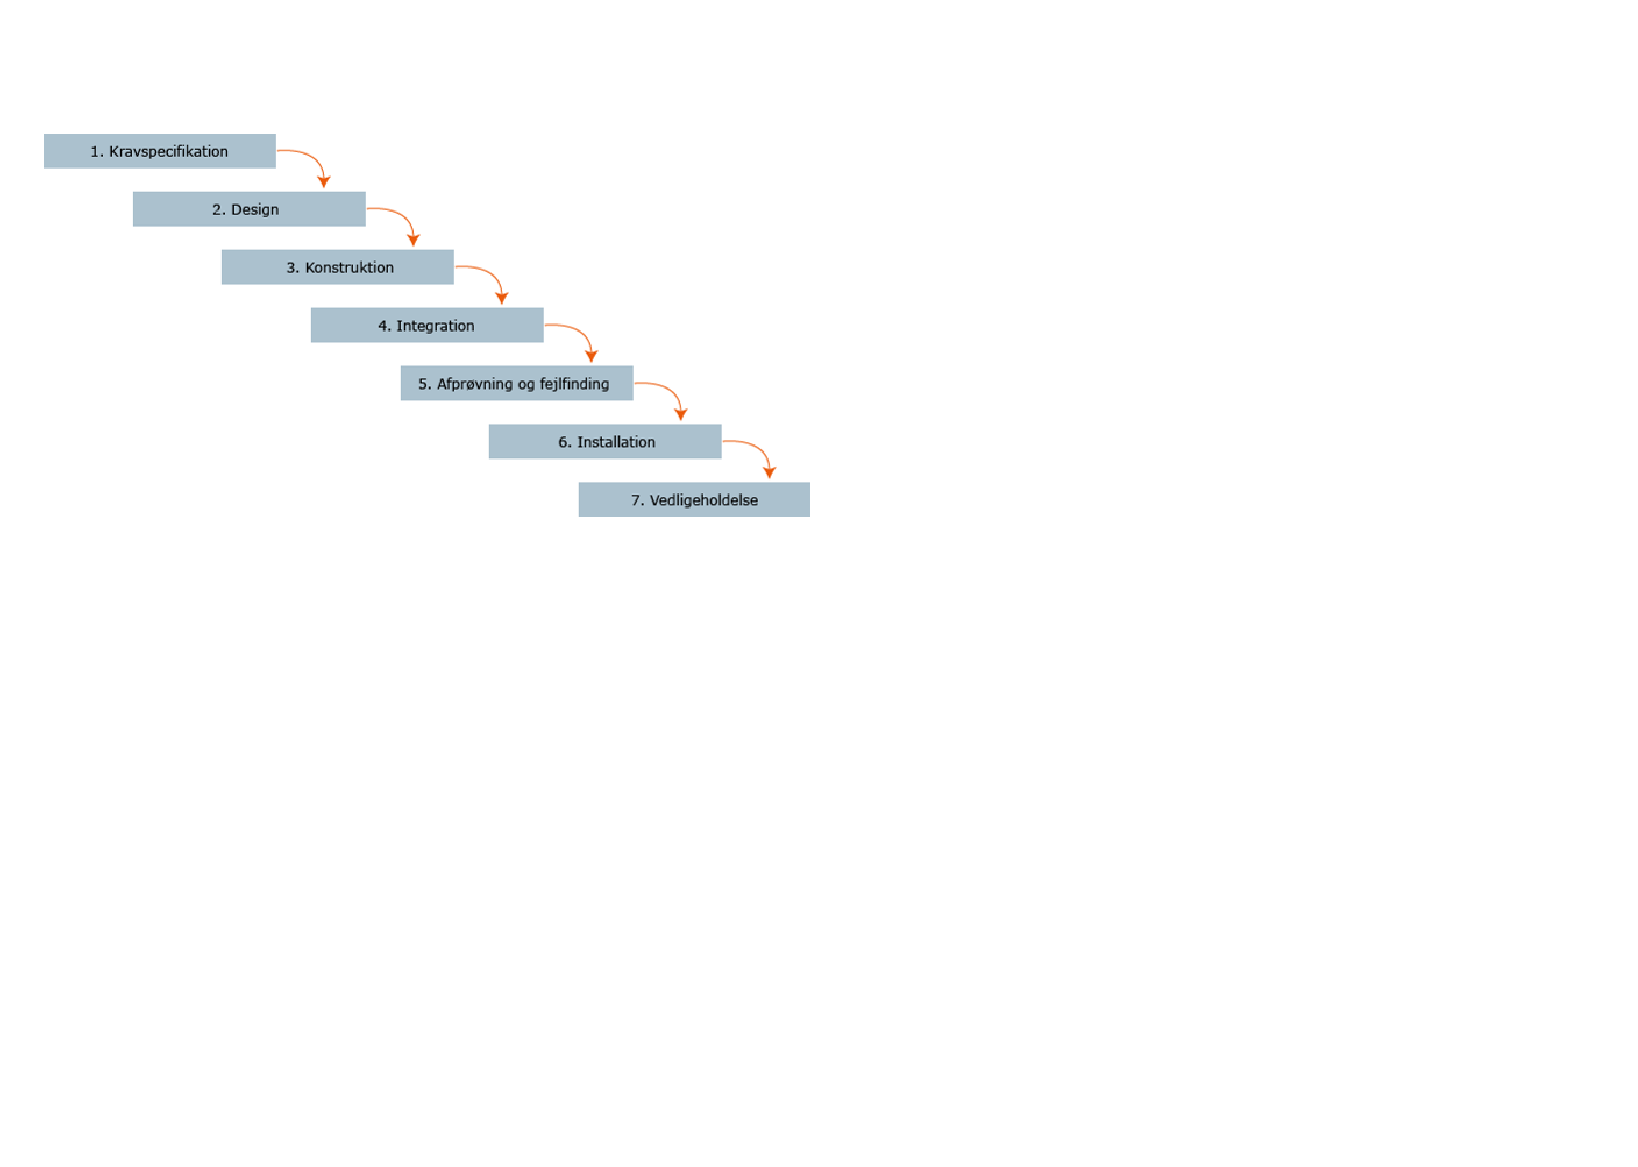
\includegraphics[clip, trim = 0mm 100mm 100mm 10mm, scale = 1]{./vandfaldmodel.eps}
\caption{Vandfaldsmodellen}
\label{dia:Vandfald}
\end{center}
\end{figure}

Essensen ved vandfaldsmodellen er, at man først kan fortsætte til næste fase i udviklingen, når den fase man er i er helt færdig. Det er vigtigt her, at bemærke i figur \ref{dia:Vandfald}, at der først testes efter udviklingen i projektet. Dette har for eksempel den konsekvens, at projektet er færdiglavet, men ikke er blevet testet igennem, for eventuelle fejl og mangler, og denne udviklingsmetode gør ikke brug af at springe tilbage i faserne, når de først er blevet lavet.
Det vil sige, at når konstruktionsfasen er færdig, kan man ikke gå tilbage og ændre i den, uanset hvad for eksempel resultatet af testfasen viser. Denne metode er oftest brugt ved kortere projekter, hvor kravene er meget specifikke og der er så få parametre udefra som muligt, der kan gå ind og ændre ved projektet.\\


\section{Scrum}
Scrum-metoden er en agil udviklingsmetode, som er særligt kendt for dets tilpasning til software udvikling, men også kan bruges i andre projekt sammenhæng og er anerkendt som et agile projektstyringsredskab. Denne metode er, i stedet for faser, opdelt i roller, hvor hver rolle indebære forskelligt ansvar.\cite{ScrumRoles} \\ \\
I forhold til andre projektmetoder, har denne ikke nogen leder, men hver person som er en del af Scrum-teamet, har lige meget ansvar. Dog skal der være en såkaldt Scrum Master, hvis ansvar er at have kontakt til Product Owner og sørge for, at Development Teamet er på rette spor med hensyn til udviklingen, tidsplaner med mere, og overholder de forskellige scrum regler der findes. Processen i denne metode, bliver styret ved hjælp af en såkaldt Product Backlog, som indeholder opgaver for hele projektet. Det er så op til Product Owner og Scrum Masteren, at finde ud af hvilke opgaver, der skal laves. For at have et overblik over arbejdsopgaverne, er der lavet såkaldte Sprints, som er arbejdsperioder i et projekt. For hvert Sprint, skal de arbejdsopgaver der er i disse laves færdige, så der opretholdes og overholdes deadlines for projektet. Dette er væsentligt for Scrum metoden, da efter hvert endt Sprint, gerne skal være et produkt, som kan lanceres. En af fordelene ved Scrum er, at der er fokus på at lancere en udgave af produktet kontinuerligt og blive ved med at komme med nye og bedre udgaver af et produkt, så længe det stadig er under udvikling. En af ulemperne ved Scrum kan være, at det er svært for Scrum Masteren at planlægge og strukturere projektet, uden en klar definition på, hvordan det endelige produkt skal se ud, da metoden gør det muligt for Product Owneren at komme med ændringer, som skal implementeres eller ændres i projektet, mellem de forskellige Sprints.\cite{SCRUM}\\
\\
\section{Unified Process (UP)}
Unified Process er også en iterativ og trinvis udviklingsmetode. Metoden består af forskellige iterationer, som hver omhandler deres emne og sætter fokus på bestemte faser i projektet. Faserne er Inception, Elaboration, Construction og Transition, som hver kan være delt op i flere individuelle iterationer alt efter størrelsen på projektet.\cite{UP}

\begin{figure}[!h]
\centering
\begin{center}
%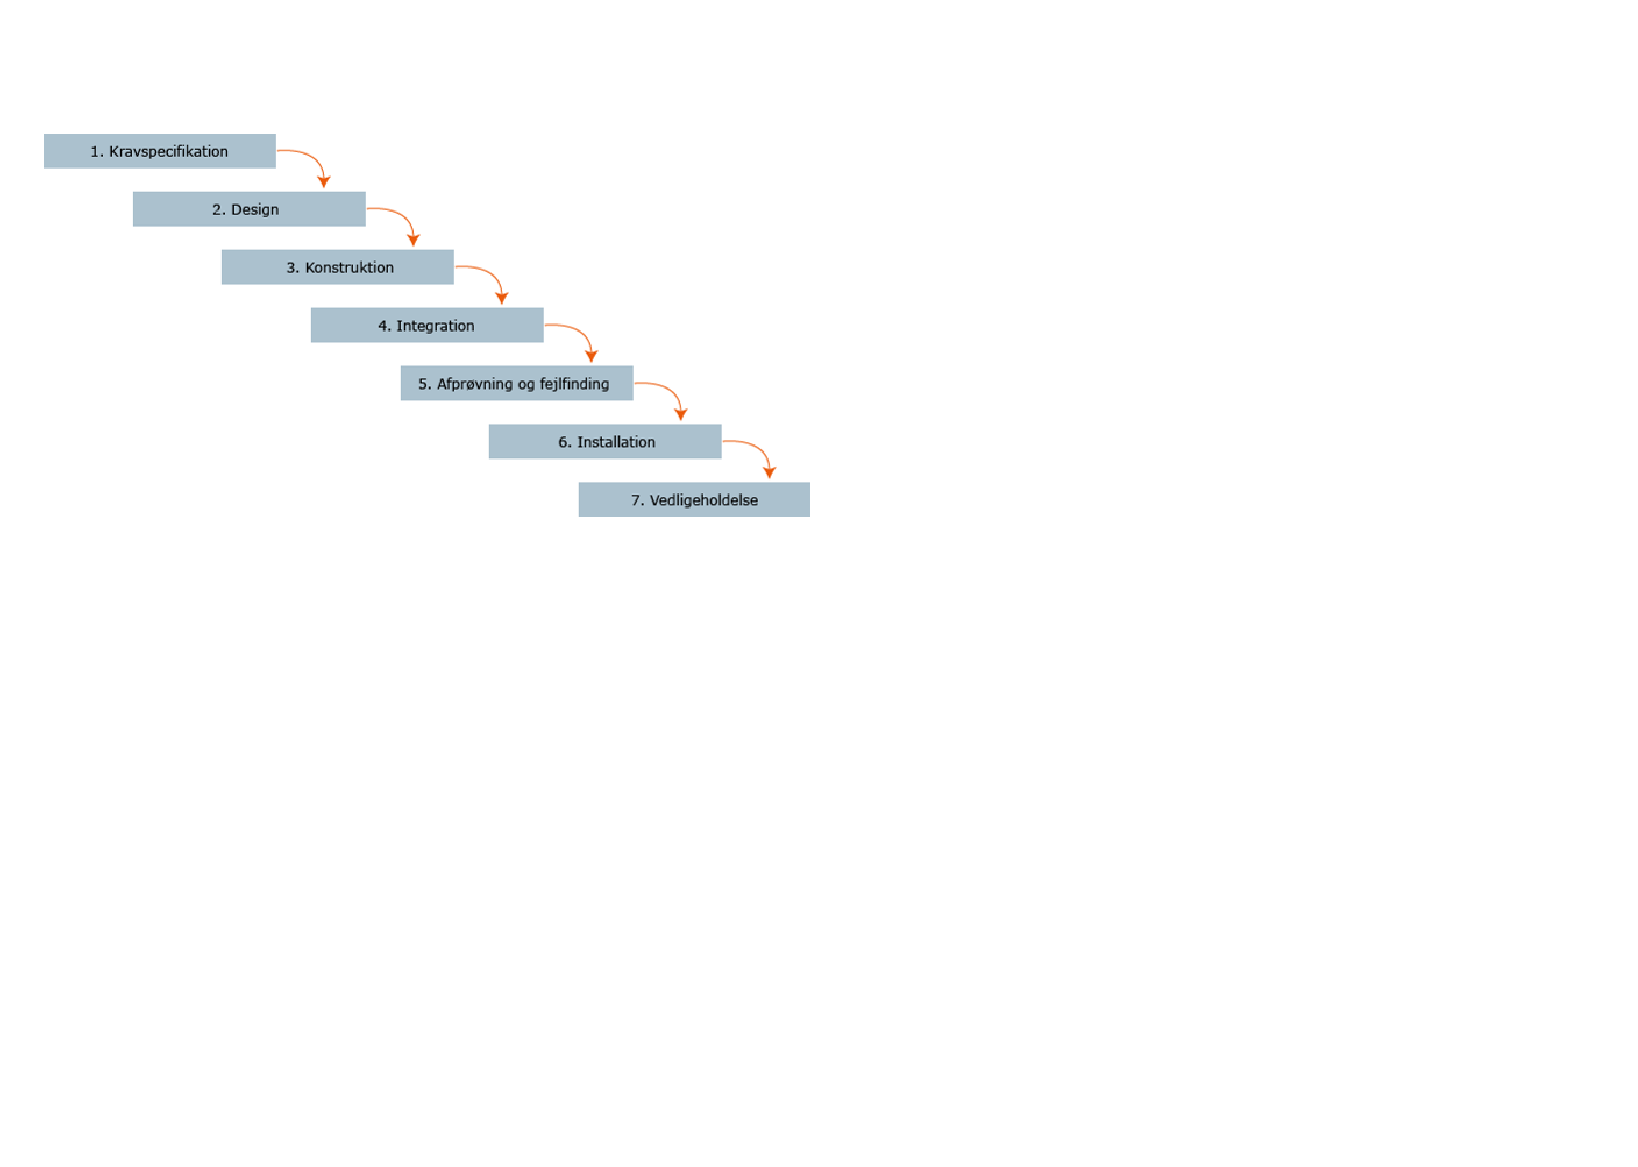
\includegraphics[scale=0.5]{./vandfaldmodel.eps}
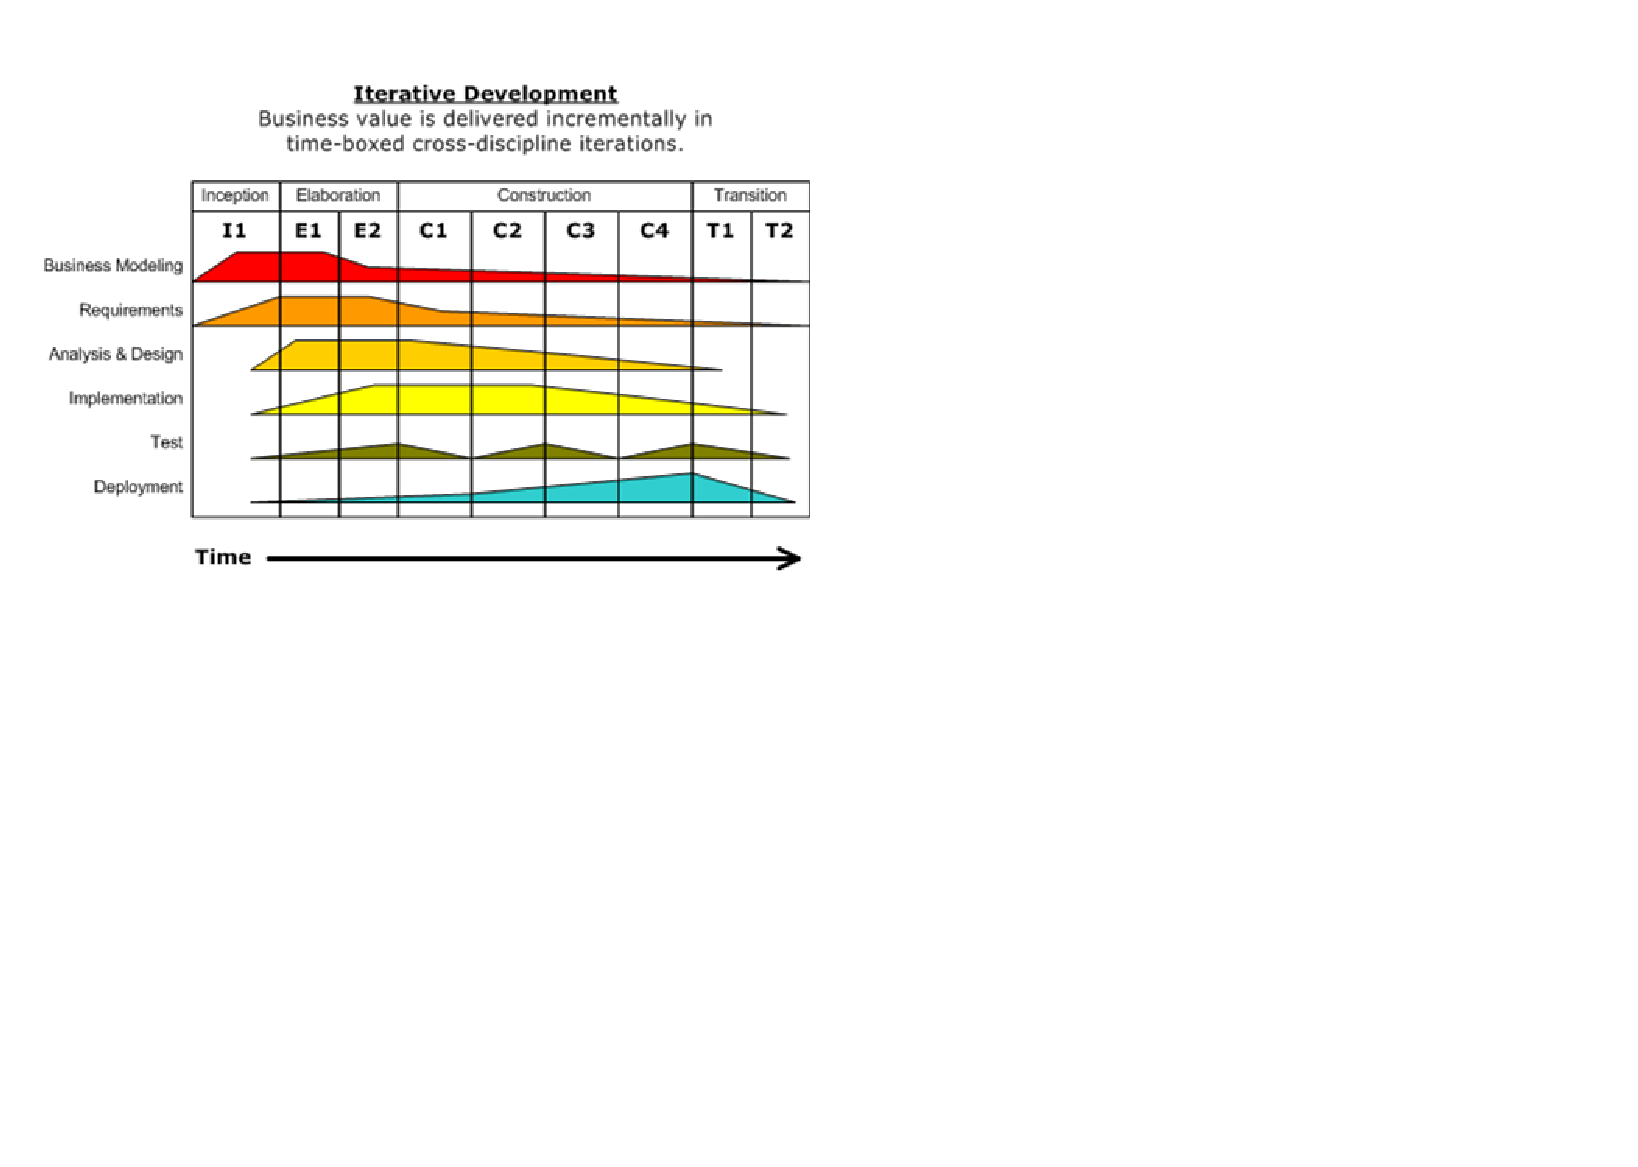
\includegraphics[clip, trim = 0mm 100mm 125mm 10mm, scale = 0.8]{./UPmetode.eps}
\caption{UP - Iterativ udviklingsmetode}
\label{dia:Iterativ}
\end{center}
\end{figure}

Metoden gør det muligt, i forhold til andre iterative metoder som Vandfaldsmodellen, at anvende iterationer, til at analysere, designe, implementere og teste i løbet af projektet, for hele tiden at forbedre og udvikle produktet. I figur \ref{dia:Iterativ}, kan ses et diagram som illustrere et eksempel på en Iterativ udviklings forløb. En af fordelene ved denne metode er, at efter hver endt iteration, så overlapper de forskellige faser hinanden, så det er muligt at gå tilbage til en fase, som tidligere var afsluttet, og tage det op i en ny iteration. En af ulemperne kan være, at det er meget Use Case drevet / Risiko drevet, da metoden afhænger meget af at man kender alle de risici faktorer, som kan spille ind i løbet af projektet. Hvis ikke alle disse findes til at starte med, kan det have en stor betydning for projektets forløb.\cite{UPPrincipper}

 %Er Udviklingsmetode-afsnittet
\cfoot{\page\textbackslash \totalp} %Skal vise x antal sider af y
%\setcounter{page}{1}
\chapter{Hvad kræver det for at holde et MMO kørende?}
Når man ser på et MMO, så er der mange ting, at tage med i overvejelserne for udviklingen. Et MMO er ofte så stort et spil, at det ikke er muligt for en enkelt programmør at holde systemet kørende selv. Dette vil sige bare i team størrelse skal man nok op omkring 100 - 200 mennesker\cite{NOMMO}, så det er svært at holde overblik og kommunikation i gang. Udover dette er der også den økonomiske side, løn til alle de programmører, penge til servere, vedligeholdelse og til eventuel videre udvikling af spillet. Der har man investorer til at hjælpe en i gang, men de penge vil de helst have tilbage igen. Til at hjælpe spilfirmaet med det har man heldigvis spillere, men for at betale et lån på 1 million dollars tilbage kræver det  omkring 10,000 subscribers som hver betaler 100 kr. om måneden over 2 år\cite{Escapist}, og så skal man helst have flere subscriber's end det, for at kunne vedligeholde omkostningerne. Det er lidt en ond cirkel når det kommer til det punkt. Der er brug for subscribers for, at skaffe penge til server vedligeholdelse, men serverne skal holdes vedlige for at spillerne. Hvis det går godt for spillet når der kommer der et overskud  ud af den anden ende, og cirklen er hermed brudt.
\chapter{Hvad er vigtigt at vedligeholde i et MMO?}
Ofte når man spiller et online spil kommer der patches eller hotfixes ind i spil, som skal løse nogle problemer der er med spillet, eller udvide det der er i spillet. Disse problemer der kan komme i driften af ens produkt kan ofte findes af testere, men nogle gange ender det med at fejlene kommer helt ud i en endelig udgave, hvor det bliver nødvendigt at hotfixe problemet. Derfor er det vigtigt at lytte til den feedback spillerne af ens produkt kommer med, så man altid kan tilfredsstille både kunder, og evt. nye kunder.\\
Når man vedligeholder et MMO er det også vigtigt at komme med nye ting spilleren kan lave, som nyt content, eller noget så simpelt som nye skins til ens avatar, så spilleren har noget at lave, og de bliver ved med at have interesse i ens produkt.\cite{WoW}\\
Man skal dog ikke kun lytte til kunder, men man skal også holde dem informeret om planer for fremtiden, og hvad de kan forvente der bliver lavet til spillet. Dette gør spil som Shroud of the Avatar\cite{SOTA}, hvor de kommer med månedlige opdateringer om hvad de har fået lavet, og hvad de kommer til at lave det næste stykke tid\cite{SOTAForum}. Dette medfølger også at man skal være aktive på sociale medier, og man skal svare på folks kritik, og lytte til hvad de siger om disse planer, og bare generelt hjælpe dem\cite{GreatMMO}. For hvis du har et godt community, så skal de nok bakke op om dit spil, selvom der bliver taget en upopulær beslutning.\cite{MMOChampion}

\cfoot{\page\textbackslash \totalp} %Skal vise x antal sider af y
\chapter{Konklusion}
I forhold til de problemstillinger der er ved at holde driften i et MMO, hvor der hele tiden kan være behov for ændringer og vedligeholdelse af forskellige dele af spillet vil en udviklingsmetode, der er flexible, være bedre egnet end en udviklingsmetode, der har faste rammer.\\
\\
Efter vores research omkring emnet, mener vi at Scrum er den bedste måde at vedligeholde et spil på. Hvis man kigger på Scrum er det hele nemlig sat op i sprints, som ville være fordelagtige i vedligeholdelsen, da man kan planlægge fremad, med hvad der skal laves på eventuelle expansions, eller hvad der skal fixes i det spil man allerede har. På denne måde kan man også informere communitiet om det man laver, imens man laver det, og derved kan man altid få feedback på det man laver. Da scrum også er en agil metode kan der komme løbende ændringer og dette er optimalt for vedligeholdelsen af et produkt. Samtidig er det muligt at kunne reagere på hvad folk har af input og lave om på ting, som måske troede ville virke, eller selv synes var en god idé, men viste sig ikke at være så god når det kom til stykket.\\
\\
Vi mener derimod også at vandfaldsmodellen ville være den mindst effektive til at vedligeholde et spil, da hvis man opdager fejl i det endelige produkt, ville man skulle gå helt tilbage til designfasen, og så tjekke op derfra om der er lavet fejl, og rette det trin for trin, i stedet for at kunne hoppe direkte ind i koden og rette den linje kode, der kunne give fejlen.\\
\\
Med henblik på vedligeholdelse, er det situations bestemt hvilken metode der vil være bedst at bruge. For eksempel hvis man har en klasse, der kunne være en spilbar Race eller et våben, som er meget bedre end de andre alternativer i spillet, kan det være mere relevant at bruge vandfaldsmodellen, da den går helt tilbage til analyse- og designfasen og tager hele problematikken op igen. Hvorimod en Scrum metode ligger an til meget mere test og måske først ville gå ind og lave små ændringer og teste det igen, til problemet er løst.\\
\\
Alle udviklingsmetoderne, som er gennemgået i denne artikel har alle sine fordele og ulemper, som skal tages hensyn til, når man vælger hvilken man vil gå ud fra når man ser hvad problemstillingen er. 


\label{lastreportpage}

\appendix
\printbibliography[heading = bibintoc] %Indsætter kildeliste
\newcounter{appendixstart}
%Til kilder
%stuff
%Dette er BILAG!!!
\chapter{Tabel: 1}
\label{tab:Penge}
\begin{tabularx}{0.75\textwidth}{|X|X|X|X|X|}
\hline
År & Budget & Resultat & Måneder at betale tilbage & År at betale tilbage \\ \hline \hline
1000 & 5000000 & 100000 & 50 & 4.2 \\ \hline
3000 & 5000000 & 300000 & 16.7 & 1.4 \\ \hline
5000 & 5000000 & 500000 & 10 & 0.8 \\ \hline
8000 & 5000000 & 800000 & 6.3 & 0.5 \\ \hline
10000 & 5000000 & 1000000 & 5 & 0.4 \\ \hline
\end{tabularx}


% USED FOR COUNTING THE NUMBER OF PAGES
\newpage
Empty page used for counting...
%\addtocounter{page}{-\value{appendixstart}}
\addtocounter{page}{-\value{appendixstart}}
\addtocounter{page}{-11}{} %-1 fordi den trækker den ekstra side fra og -10 for de sider der er i reporten.
\label{lastappendixpage}
\newpage
Empty page used for counting...
%\addtocounter{page}{10}{}
\addtocounter{page}{\value{totalp}}
\addtocounter{page}{+9}{} %+11 for at komme op på det normale sidetal og -2, for de ekstra sider der er lavet.
\label{totalpages}
\mbox{}

\end{document}